\documentclass[../../main.tex]{subfiles}
\graphicspath{{\subfix{../../image/}}} % 指定图片目录,后续可以直接使用图片文件名。

% 例如:
% \begin{figure}[H]
% \centering
% \includegraphics[scale=0.4]{图.png}
% \caption{}
% \label{figure:图}
% \end{figure}
% 注意:上述\label{}一定要放在\caption{}之后,否则引用图片序号会只会显示??.

\begin{document}

\section{可测函数列的收敛}

\subsection{几乎处处收敛与一致收敛}

\begin{definition}[几乎处处收敛]
设$f(x), f_1(x), f_2(x), \cdots, f_k(x), \cdots$是定义在点集$E \subset \mathbb{R}^n$上的广义实值函数。若存在$E$中的点集$Z$,有$m(Z) = 0$及
\begin{align*}
\lim_{k \to \infty} f_k(x) = f(x), \quad x \in E \setminus Z,
\end{align*}
则称$\{f_k(x)\}$在$E$上\textbf{几乎处处收敛}于$f(x)$,并记为
\begin{align*}
f_k(x) \to f(x),\,\text{a. e. } x \in E.
\end{align*}
或
\begin{align*}
\lim_{k \to \infty} f_k(x) = f(x),\,\text{a.e.}\, x \in E.
\end{align*}
再不引起歧义下,也可简记为
\begin{align*}
f_k\xrightarrow{\mathrm{a}.\mathrm{e}.}f.
\end{align*}
\end{definition}

\begin{theorem}
若$\{f_k(x)\}$是$E$上的可测函数列,并且$f_k(x) \to f(x),\text{a. e.} x \in E.$则$f(x)$也是$E$上的可测函数。
\end{theorem}
\begin{proof}
由条件可知\(\{ f_k(x) \}\)是\(E\)上的可测函数列,并且$Z$为零测集也可测,从而\(E\backslash Z\)是可测集.于是由\nrefthe{theorem:定理3.3}{(2)}可知\(\{ f_k(x) \}\)是\(E\backslash Z\)上的可测函数列,并且由条件可知\(\lim_{k\rightarrow \infty}f_k(x) =f(x) \ (x\in E\backslash Z)\),因此由\refcor{corollary:可测函数列的极限也可测}可得\(f(x)\)也是\(E\backslash Z\)上的可测函数。又注意到对\(\forall t\in \mathbb{R}\),都有
\begin{align*}
\{ x\in Z:f (x) >t \} \subset Z.
\end{align*}
而Z是零测集,由\hyperref[proposition:零测集的基本性质]{零测集的子集也是零测集}可知,\(\left\{ x\in Z:f(x) >t \right\}\)也是零测集,从而\(\left\{ x\in Z:f(x) >t \right\}\)也可测。于是\(f(x)\)在Z上可测。故由\nrefthe{theorem:定理3.3}{(1)}可知\(f(x)\)在\(E=(E\backslash Z)\cup Z\)上可测。
\end{proof}

\begin{definition}[(接)近一致收敛]
设 $\{f_n(x)\}$ 为 $E$ 上的可测函数列,对 $\forall\delta > 0$,存在可测子集$E_\delta\subset E$:$m(E_\delta) < \delta$,使得 $\{f_n(x)\}$ 在 $E\backslash E_\delta$ 上一致收敛于 $f(x)$,
则称 $\{f_n(x)\}$ 在 $E$ 上\textbf{(接)近一致收敛}于 $f(x)$. 

这也等价于,
对$\forall \delta >0$,存在$E$的可测子集$F_\delta\subset E$:$m(E\backslash F_\delta)<\delta$,使得$\{f_k(x)\}$在$F_\delta$上一致收敛于$f(x)$.
\end{definition}
\begin{remark}
上述两个等价定义的证明:$\Rightarrow$:对$\forall \delta >0$,只需令$F_\delta=E\backslash E_\delta$,则显然$F_\delta$为$E$的可测子集,且$E_\delta=E\backslash F_\delta$.从而$m(E\backslash F_\delta)=m(E_\delta)<\delta$且$\{f_k(x)\}$也在$E\backslash E_\delta=F_\delta$上一致收敛于$f(x)$.
$\Leftarrow$:对$\forall \delta >0$,取$E_\delta=E\backslash F_\delta$,同理可证.
\end{remark}

\begin{lemma}\label{lemma:引理3.11}
设$f(x), f_1(x), f_2(x), \cdots, f_k(x), \cdots$是$E$上几乎处处有限的可测函数,且$m(E) < +\infty$。若$f_k(x) \to f(x)$, a. e. $x \in E$,则对任给$\varepsilon > 0$,令
\begin{align*}
E_k(\varepsilon) = \{x \in E: |f_k(x) - f(x)| \geqslant \varepsilon\},
\end{align*}
则$E_k(\varepsilon)(k=1,2,\cdots)$可测,并且
\begin{align}
\lim_{j \to \infty} m\left( \bigcup_{k = j}^{\infty} E_k(\varepsilon) \right) = 0. \label{eq:3.6}
\end{align}
\end{lemma}
\begin{proof}
注意到对$\forall k\in \mathbb{N}$,都有
\begin{align*}
E_k(\varepsilon )&=\{x\in E:|f_k(x)-f(x)|\geqslant \varepsilon \}=\left\{ x\in E:-\varepsilon \leqslant f_k(x)-f(x)\leqslant \varepsilon \right\} 
\\
&=\left\{ x\in E:f_k(x)-f(x)\geqslant -\varepsilon \right\} \cup \left\{ x\in E:f_k(x)-f(x)\leqslant \varepsilon \right\} .
\end{align*}
因为$f_k(x)$和$f(x)$都在$E$上可测,所以由\hyperref[theorem:可测函数的运算性质]{可测函数的运算性质(1)}可知$f_k(x)-f(x)$也在$E$上可测.从而再由\refthe{theorem:定理3.2}及\hyperref[theorem:可测集的性质]{可测集的性质}可得
\[
E_k(\varepsilon)=\left\{ x\in E:f_k(x)-f(x)\geqslant -\varepsilon \right\} \cup \left\{ x\in E:f_k(x)-f(x)\leqslant \varepsilon \right\}\in \mathscr{M}.
\]
由函数列收敛的否命题可知,上限集$\bigcap_{j = 1}^{\infty} \bigcup_{k = j}^{\infty} E_k(\varepsilon)$中的点一定不是收敛点,从而依题设可知
\begin{align*}
m\left( \lim_{j \to \infty}\bigcup_{k = j}^{\infty} E_k(\varepsilon) \right)=m\left( \bigcap_{j = 1}^{\infty} \bigcup_{k = j}^{\infty} E_k(\varepsilon) \right) = 0.
\end{align*}
根据\hyperref[corollary:递减可测集列的测度运算]{递减可测集列的测度运算},可知\eqref{eq:3.6}式成立.
\end{proof}

\begin{theorem}[Egorov(叶戈洛夫)定理]\label{theorem:Egorov定理}
设 $f(x),f_1(x),f_2(x),\cdots,f_k(x),\cdots$ 是 $E$ 上几乎处处有限的可测函数,且 $m(E)<+\infty$,若$f_k(x)\to f(x)$, a.e. $x\in E$,则
$\{f_n(x)\}$在$E$上接近一致收敛于$f(x)$.
\end{theorem}
\begin{remark}
\hyperref[theorem:Egorov定理]{Egorov定理}中的条件 $m(E)<+\infty$ 不能去掉. 例如考虑可测函数列
\begin{align*}
f_n(x)=\chi_{(0,n)}(x),\quad n = 1,2,\cdots,\quad x\in(0,+\infty).
\end{align*}
它在 $(0,+\infty)$ 上处处收敛于 $f(x)\equiv1$,但在 $(0,+\infty)$ 中的任一个有限测度集外均不一致收敛于 $f(x)\equiv1$.

但对 $m(E)=+\infty$ 的情形,结论可陈述如下:对任给 $M>0$,存在 $E_M$:$E_M\subset E$,$m(E_M)>M$,使得 $f_n(x)$ 在 $E_M$ 上一致收敛于 $f(x)$.(见\refcor{corollary:Egorov定理(当E为无穷测度集时)})
\end{remark}
\begin{proof}
由\reflem{lemma:引理3.11}可知,对任给的 $\varepsilon>0$,有
\begin{align*}
\lim_{j\to\infty}m\left(\bigcup_{k = j}^{\infty}E_k(\varepsilon)\right)=0.
\end{align*}
其中$E_k(\varepsilon) = \{x \in E: |f_k(x) - f(x)| \geqslant \varepsilon\}$可测.
现在取正数列 $1/i$ ($i = 1,2,\cdots$),则对任给的 $\delta>0$ 以及每一个 $i$,存在 $j_i$,使得 $m\left(\bigcup_{k = j_i}^{\infty}E_k\left(\frac{1}{i}\right)\right)<\frac{\delta}{2^i}$. 令 $E_\delta=\bigcup_{i = 1}^{\infty}\bigcup_{k = j_i}^{\infty}E_k\left(\frac{1}{i}\right)$,显然$E_\delta$可测.我们有
\begin{align*}
m(E_\delta)\leqslant\sum_{i = 1}^{\infty}m\left(\bigcup_{k = j_i}^{\infty}E_k\left(\frac{1}{i}\right)\right)\leqslant\sum_{i = 1}^{\infty}\frac{\delta}{2^i}=\delta.
\end{align*}
现在来证明在点集
\begin{align*}
E\backslash E_\delta=\bigcap_{i = 1}^{\infty}\bigcap_{k = j_i}^{\infty}\left\{x\in E:\vert f_k(x)-f(x)\vert<\frac{1}{i}\right\}
\end{align*}
上,$\{f_k(x)\}$ 是一致收敛于 $f(x)$ 的.

事实上,对于任给 $\varepsilon>0$,存在 $i$,使得 $1/i<\varepsilon$,从而对一切 $x\in E\backslash E_\delta$,当 $k\geqslant j_i$ 时,有
\begin{align*}
\vert f_k(x)-f(x)\vert<\frac{1}{i}<\varepsilon.
\end{align*}
这说明 $f_k(x)$ 在 $E\backslash E_\delta$ 上一致收敛于 $f(x)$. 
\end{proof}

\begin{theorem}[Egorov(叶戈洛夫)定理的逆定理]\label{theorem:Egorov定理的逆定理}
设 $\{f_n(x)\}$ 是 $E$ 上的可测函数,若$\{f_n(x)\}$在$E$上接近一致收敛于$f(x)$,则$f_k(x)\to f(x)$, a.e. $x\in E$.
\end{theorem}
\begin{proof}
分别取 $\delta_k = 1/k$,$k = 1,2,\cdots$,则存在 $F_k\subset E$,$m(F_k)<1/k$,使得$f_n(x)$在每个$E\backslash F_k$上均一致收敛于$f(x)$.
记 $F = \bigcap_{k = 1}^{\infty}F_k$,则$F$可测,且
\[
m(F)\leqslant m(F_k)<\frac{1}{k},\quad k = 1,2,\cdots
\]
令 $k\to\infty$ 得 $m(F) = 0$. 下面证明 $f_k(x)$ 在 $E\backslash F$ 上处处收敛于 $f(x)$.

由于
\begin{align*}
E\backslash F=E\backslash \bigcap_{k = 1}^{\infty}F_k=E\cap\left(\bigcup_{k = 1}^{\infty}F_k^c\right)
=\bigcup_{k = 1}^{\infty}(E\cap F_k^c)=\bigcup_{k = 1}^{\infty}(E\backslash F_k).
\end{align*}
故对 $\forall x_0\in E\backslash F$,存在 $k_0\in\mathbb{N}$,使得 $x_0\in E\backslash F_{k_0}$. 又 $f_k$ 在 $E\backslash F_{k_0}$ 上一致收敛于 $f$,从而$\lim_{k\to \infty}f_k(x)=f(x),\forall x\in E\backslash F_{k_0}$,于是$\lim_{k\to \infty}f_k(x_0)=f(x_0)$.故由$x_0$的任意性可得$f_k(x)$ 在 $E\backslash F$ 上处处收敛于 $f(x)$.综上可知,$f_k(x)\to f(x)$, a.e. $x\in E$.
\end{proof}

\begin{corollary}\label{corollary:Egorov定理(当E为无穷测度集时)}
设 $f(x),f_1(x),f_2(x),\cdots,f_k(x),\cdots$ 是 $E$ 上几乎处处有限的可测函数,且 $m(E)=+\infty$. 若 $f_k(x)\to f(x)$,a.e. $x\in E$,则对任给 $M>0$,存在 $E_M$:$E_M\subset E$,$m(E_M)>M$,使得 $f_k(x)$ 在 $E_M$ 上一致收敛于 $f(x)$.
\end{corollary}
\begin{proof}
令 $E_k=E\cap B(0,k)$,显然 $\{E_k\}$ 为递增可测集列,并且
\begin{align*}
m(E_k)\leqslant m(B(0,k))<+\infty.
\end{align*}
又 $m(E)=+\infty$,故
\begin{align}
\lim_{k\rightarrow\infty}m(E_k)\xlongequal{\text{\hyperref[theorem:递增可测集列的测度运算]{递增可测集列的测度运算}}}m(\lim_{k\rightarrow\infty}E_k)=m\left(\bigcup_{k = 1}^{\infty}E_k\right)=m(E)=+\infty.\label{eq:100.68}
\end{align}
因为 $f_k(x)$($k = 1,2,\cdots$)和 $f(x)$ 在 $E$ 上可测,所以由\nrefthe{theorem:定理3.3}{(2)} 可知 $f_k(x)$($k = 1,2,\cdots$)和 $f(x)$ 在 $E_k$($k = 1,2,\cdots$)上也可测. 于是在 $E_k$ 上应用 \hyperref[theorem:Egorov定理]{Egorov 定理}可得,对 $\forall k\in\mathbb{N}$,存在可测子集 $F_k\subset E_k$,且 $m(E_k\backslash F_k)<\frac{1}{k}$,使得 $\{f_k(x)\}$ 在每个$F_k$ 上均一致收敛于 $f(x)$.从而由$m(E_k\backslash F_k)<\frac{1}{k}$ 可得
\begin{align*}
m(F_k)>m(E_k)-\frac{1}{k}.
\end{align*}
令 $k\rightarrow +\infty$,再结合 \eqref{eq:100.68} 式可得 $\lim_{k\rightarrow\infty}m(F_k)=+\infty$. 因此,对 $\forall M>0$,存在 $k\in\mathbb{N}$,使得 $m(F_k)>M$. 故取 $E_M=F_k$ 即得结论. 
\end{proof}

\begin{corollary}
设 $\{f_n(x)\}$ 以及 $f(x)$ 均是 $E$ 上几乎处处有限的可测函数,且有 $f_n(x)\to f(x)$,a.e. $x\in E$,则存在可测集列 $\{E_i\}$:$E_i\subset E$ ($i\in\mathbb{N}$),且
\begin{align*}
m\left(E\backslash\bigcup_{i = 1}^{\infty}E_i\right)=0,
\end{align*}
使得 $f_n(x)$ 在每个 $E_i$ 上均一致收敛于 $f(x)$. 
\end{corollary}
\begin{proof}
(1)当$m(E)<+\infty$时,对 $\forall i\in \mathbb{N}$,根据\hyperref[theorem:Egorov定理]{Egorov定理},取 $\delta _i=\frac{1}{i}>0$,则存在可测子集 $E_i\subset E$,使得 $m\left( E\backslash E_i \right) <\frac{1}{i}$,并且 $\left\{ f_n\left( x \right) \right\}$ 在 $E_i$ 上一致收敛于 $f\left( x \right)$.注意到对 $\forall i\in \mathbb{N}$,都有
\begin{align*}
E\backslash \bigcup_{i=1}^{\infty}{E_i}\subset E\backslash E_i,
\end{align*}
因此
\begin{align*}
m\left( E\backslash \bigcup_{i=1}^{\infty}{E_i} \right) \leqslant m\left( E\backslash E_i \right) <\frac{1}{i},\quad \forall i\in \mathbb{N}.
\end{align*}
再令 $i\rightarrow +\infty$ 得
\begin{align*}
m\left( E\backslash \bigcup_{i=1}^{\infty}{E_i} \right) =0.
\end{align*}

(2)当$m(E)=+\infty$时,令
\begin{align*}
A_1=E\cap B(0,1),
A_k=E\cap (B(0,k)\backslash B(0,k - 1))(k = 2,3,\cdots),
\end{align*}
显然 $\{A_k\}$ 是一列互不相交的可测集,满足 $A_k\subset E$,$m(A_k)<+\infty$ 且 $\bigcup_{k = 1}^{\infty}A_k=E$.

对 $\forall k\in\mathbb{N}$,考虑 $A_k$,则由 $(1)$ 可知,存在可测集列 $\{E_{k,i}\}$:$E_{k,i}\subset E$($i\in\mathbb{N}$)且
\begin{align}
m\left( A_k\backslash \bigcup_{i = 1}^{\infty}E_{k,i} \right) = 0,\label{eq:100.70}
\end{align}
使得 $\{f_n(x)\}$ 在每个 $E_{k,i}$($\forall i\in\mathbb{N}$)上均一致收敛于 $f(x)$. 进而再由 $k$ 的任意性可得,$\{f_n(x)\}$ 在每个 $E_{k,i}$($\forall k,i\in\mathbb{N}$)上均一致收敛于 $f(x)$. 考虑集族 $\mathcal{F}=\{E_{k,i}|k,i\in\mathbb{N}\}$. 由于 $\mathbb{N}\times\mathbb{N}$ 可数,故 $\mathcal{F}$ 也可数. 因此可将 $\mathcal{F}$ 枚举为序列 $\{E_i\}_{i = 1}^{\infty}$. 故 $\{f_n(x)\}$ 在每个 $E_i$($\forall i\in\mathbb{N}$)上均一致收敛于 $f(x)$. 由\refthe{theorem:集族的并和交的基本性质}可知
\begin{align}
\bigcup_{k = 1}^{\infty}A_k\backslash \bigcup_{k = 1}^{\infty}\bigcup_{i = 1}^{\infty}E_{k,i}\subset \bigcup_{k = 1}^{\infty}\left( A_k\backslash \bigcup_{i = 1}^{\infty}E_{k,i} \right).\label{eq:100.71}
\end{align}
又由 $\{A_k\}$ 互不相交可得
\begin{align}
\left( A_k\backslash \bigcup_{i = 1}^{\infty}E_{k,i} \right) \cap \left( A_l\backslash \bigcup_{i = 1}^{\infty}E_{l,i} \right) =\varnothing,k\ne l.\label{eq:100.72}
\end{align}
故利用 \eqref{eq:100.70}\eqref{eq:100.71}\eqref{eq:100.72} 式可得
\begin{align*}
m\left( E\backslash \bigcup_{i = 1}^{\infty}E_i \right) =m\left( \bigcup_{k = 1}^{\infty}A_k\backslash \bigcup_{k = 1}^{\infty}\bigcup_{i = 1}^{\infty}E_{k,i} \right) 
\leqslant m\left( \bigcup_{k = 1}^{\infty}\left( A_k\backslash \bigcup_{i = 1}^{\infty}E_{k,i} \right) \right) 
=\sum_{k = 1}^{\infty}m\left( A_k\backslash \bigcup_{i = 1}^{\infty}E_{k,i} \right)=0.
\end{align*} 
\end{proof}

\begin{example}
考查 $f_n(x)=x^n$($0\leqslant x\leqslant1$),$f(x)=0$($0\leqslant x<1$)以及 $f(1)=1$,则在 $[0,1]$ 上 $f_n(x)$ 点收敛于 $f(x)$ 而非一致收敛于 $f(x)$. 但在舍去一个测度可任意小的正测集(如 $(1 - \delta,1]$)后,$f_n(x)$ 在余下点集上一致收敛于 $f(x)$. 
\end{example}
\begin{proof}

\end{proof}



\subsection{几乎处处收敛与依测度收敛}

\begin{definition}
设 $f(x),f_1(x),f_2(x),\cdots,f_k(x),\cdots$ 是 $E$ 上几乎处处有限的可测函数. 若对任给的 $\varepsilon>0$,有
\begin{align}
\lim_{k\to\infty}m(\{x\in E:\vert f_k(x)-f(x)\vert \geqslant \varepsilon\}) = 0,\label{eq:3.7}
\end{align}
或等价地,若对 $\forall\varepsilon > 0$ 及 $\delta > 0$,存在 $N_{\varepsilon,\delta}\in\mathbb{N}$,使得当 $n\geqslant N_{\varepsilon,\delta}$ 时,有 $m(E_n(\varepsilon)) < \delta$,则称 $\{f_k(x)\}$ 在 $E$ 上\textbf{依测度收敛于}$f(x)$,简记为 $f_n\stackrel{\mu}{\longrightarrow}f$. 
\end{definition}
\begin{remark}
注意,由$f_k(x)$在$E$上几乎处处有限可知$m(\{x\in E:\vert f_k(x)\vert=+\infty\}) = 0\quad (k = 1,2,\cdots)$. 
\end{remark}

\begin{theorem}\label{theorem:依测度收敛的极限函数必唯一}
若 $\{f_k(x)\}$ 在 $E$ 上同时依测度收敛于 $f(x)$ 与 $g(x)$,则 $f(x)$ 与 $g(x)$ 是对等的.
\end{theorem}
\begin{note}
这个定理告诉我们:在函数对等的意义下,依测度收敛的极限函数是唯一的.
\end{note}
\begin{proof}
因为对$\forall x\in E$,有
\begin{align*}
\vert f(x)-g(x)\vert\leqslant\vert f(x)-f_k(x)\vert+\vert g(x)-f_k(x)\vert,
\end{align*}
所以对任给 $\varepsilon>0$,有
\begin{align*}
&\{x\in E:\left| f(x)-g(x) \right|\geqslant \varepsilon \}\subset \left\{ x\in E:\left| f\left( x \right) -f_k\left( x \right) \right|+\left| g\left( x \right) -f_k\left( x \right) \right|\geqslant \varepsilon \right\} 
\\
&=\left\{ x\in E:\left| f(x)-f_k(x) \right|\geqslant \frac{\varepsilon}{2} \right\} \cup \left\{ x\in E:\left| g(x)-f_k(x) \right|\geqslant \frac{\varepsilon}{2} \right\} .
\end{align*}
但当 $k\to\infty$ 时,上式右端点集的测度趋于零,从而得
\begin{align*}
m(\{x\in E:\vert f(x)-g(x)\vert\geqslant \varepsilon\}) = 0.
\end{align*}
由 $\varepsilon$ 的任意性可知 $f(x)=g(x)$,a.e. $x\in E$. 
\end{proof}

\begin{theorem}\label{theorem:依测度收敛的极限函数必几乎处处有限}
设\(\{f_k(x)\}\)在\(E\)上几乎处处有限,若\(\{f_k(x)\}\)在\(E\)上依测度收敛于\(f(x)\),则\(f(x)\)几乎处处有限。
\end{theorem}
\begin{proof}
设\(A = \{x \in E : |f(x)| = +\infty\}\),则只需证\(m(A) = 0\)。由于每个\(f_k(x)\)在\(E\)上几乎处处有限,因此对\(\forall k \in \mathbb{N}\),令\(B_k = \{x \in E : |f_k(x)| = +\infty\}\),则\(m(B_k) = 0\)。
再令\(B = \bigcup_{k=1}^{\infty} B_k\),则\(B\)是可数个零测集的并,而零测集必可测,故\(B\)也可测。并且
\begin{align*}
m(B) \leqslant \sum_{k=1}^{\infty} m(B_k) = 0.
\end{align*}
因此\(m(B) = 0\)。对\(\forall x_0 \in A \setminus B\),都有
\begin{align*}
|f(x_0)| = +\infty, \quad |f_k(x_0)| < +\infty.
\end{align*}
于是对\(\forall \varepsilon > 0\),\(k \in \mathbb{N}\),都有
\begin{align*}
|f_k(x_0) - f(x_0)| \geqslant \varepsilon.
\end{align*}
这表明对\(\forall \varepsilon > 0\),\(k \in \mathbb{N}\),都有\(x_0 \in \{x \in E : |f_k(x) - f(x)| \geqslant \varepsilon\}\)。再由\(x_0\)的任意性可得
\begin{align*}
A \setminus B \subset \{x \in E : |f_k(x) - f(x)| \geqslant \varepsilon\}, \quad \forall \varepsilon > 0, \, k \in \mathbb{N}.
\end{align*}
从而再结合\(m(B) = 0\)可得
\begin{align*}
m(A) = m(A \setminus B) \leqslant m(\{x \in E : |f_k(x) - f(x)| \geqslant \varepsilon\}), \quad \forall \varepsilon > 0, \, k \in \mathbb{N}.
\end{align*}
令\(k \to \infty\)可得
\begin{align*}
m(A) \leqslant \lim_{k \to \infty} m(\{x \in E : |f_k(x) - f(x)| \geqslant \varepsilon\}).
\end{align*}
又因为\(\{f_k(x)\}\)在\(E\)上依测度收敛于\(f(x)\),所以
\begin{align*}
\lim_{k \to \infty} m(\{x \in E : |f_k(x) - f(x)| \geqslant \varepsilon\}) = 0.
\end{align*}
故\(m(A) = 0\),结论得证。
\end{proof}

\begin{example}[收敛但不一致收敛的函数]

$f_n(x)=x^n$,$n = 1,2,\cdots$ 
\end{example}
\begin{proof}
显然$\{f_n(x)\}$在 $[0,1]$ 上处处收敛于
\[
f(x)=
\begin{cases}
0, & 0\leqslant x<1 \\
1, & x = 1
\end{cases}
\]
但不一致收敛于 $f(x)$,因为连续函数列的一致收敛极限必连续,而 $f(x)$ 不连续. 然而,去掉任意小的一段之后一致收敛,即:对 $\forall\delta>0$,$f_n(x)$ 在 $[0,1 - \delta]$ 上一致收敛于 $0$.
\end{proof}

\begin{example}[依测度收敛但不几乎处处收敛的函数]

对每个 $n\in\mathbb{N}$,都存在唯一的 $k,i\in\mathbb{N}$,使得
\[
n = 2^k + i,\quad 0\leqslant i<2^k
\]
定义 $[0,1]$ 上的函数
\[
f_n(x)=\chi_{[\frac{i}{2^k},\frac{i + 1}{2^k})}(x),\quad n = 1,2,\cdots
\]
\end{example}
\begin{proof}
任取 $x_0\in[0,1]$,对每个 $k\in\mathbb{N}$,$\exists 0\leqslant i_k<2^k$ 使得
\[
x_0\in\left[\frac{i_k}{2^k},\frac{i_k + 1}{2^k}\right)
\]
记 $n_k = 2^k + i_k$,则
\[
f_{n_k}(x_0)=1,\quad k = 1,2,\cdots
\]
可见,$\{f_n(x_0)\}$ 有无穷多项为 $1$,无穷多项为 $0$. 故 $f_n(x)$ 在 $[0,1]$ 上每个点都不收敛(从而不是几乎处处收敛). 但对 $\forall\varepsilon\in(0,1)$,有
\[
m\{x\in[0,1]:\vert f_n(x)-0\vert\geqslant\varepsilon\}=\frac{1}{2^k}\to 0,\quad n\to\infty
\]
其中,$n = 2^k + i$,$0\leqslant i<2^k$. 故 $f_n\stackrel{\mu}{\longrightarrow}0$. (这表明 $n$ 越大,出现 “$1$” 的频率越趋于 $0$.) 
\end{proof}

\vspace{0.4cm}

从几乎处处收敛与依测度收敛的定义可以看出,前者强调的是在点上函数值的收敛(尽管除一个零测集外),后者并非指在哪个点上的收敛,其要点在于点集
\begin{align*}
\{x\in E:\vert f_k(x)-f(x)\vert\geqslant\varepsilon\}
\end{align*}
的测度应随 $k$ 趋于无穷而趋于零,而不论此点集的位置状态如何. 这是两者的区别.下面我们讨论它们之间的联系.

\begin{theorem}[Lebesgue定理]\label{theorem:几乎处处收敛在E的测度有限前提下必依测度收敛}
设 $\{f_k(x)\}$ 是 $E$ 上几乎处处有限的可测函数列,且 $m(E)<+\infty$. 若 $\{f_k(x)\}$ 几乎处处收敛于几乎处处有限的函数 $f(x)$,则 $f_k(x)$ 在 $E$ 上依测度收敛于 $f(x)$(反之不然).
\end{theorem}
\begin{remark}
\begin{enumerate}
\item 上述定理中的条件\(m(E) < +\infty\)不能去掉. 例如,取\(E = (0, +\infty)\),令\(f_n(x) = \chi_{(0,n]}(x)\),则
\[f_n(x) \to f(x) \equiv 1, \quad x \in E\]
但当取\(\delta = 1/2 > 0\)时,有
\begin{align*}
m(\{x \in E : |f_n(x) - f(x)| \geqslant \delta\}) = m((n, +\infty)) = +\infty
\end{align*}
故\(f_n\)不依测度收敛到\(f\). 

\item 上述定理中的条件\(f(x)\)几乎处处有限也不能去掉。

例如,考虑\(E = [0, 1]\),定义函数列\(f_k(x) = k\),则\(m(E) = 1 < +\infty\),且每个\(f_k(x)\)在\(E\)上处处有限。

令\(f(x) = +\infty\),则\(\lim_{k \to \infty} f_k(x) = +\infty = f(x)\),a.e. \(x \in E\)。但对\(\forall \varepsilon > 0\),都有
\begin{align*}
|f_k(x) - f(x)| = +\infty \geqslant \varepsilon, \quad \forall x \in E.
\end{align*}
于是
\begin{align*}
\{x \in E : |f_k(x) - f(x)| \geqslant \varepsilon\} = E.
\end{align*}
从而
\begin{align*}
\lim_{k \to \infty} m(\{x \in E : |f_k(x) - f(x)| \geqslant \varepsilon\}) = m(E) = 1 \ne 0.
\end{align*}
故\(\{f_k(x)\}\)在\(E\)上不依测度收敛于\(f(x)\)。
\end{enumerate}
\end{remark}
\begin{proof}
因为题设满足\reflem{lemma:引理3.11}的条件,故对任给的 $\varepsilon>0$,可知
\begin{align*}
\lim_{k\to\infty}m\left(\bigcup_{j = k}^{\infty}\{x\in E:\vert f_j(x)-f(x)\vert\geqslant\varepsilon\}\right)=0.
\end{align*}
于是
\begin{align*}
m(\{x\in E:\left| f_k(x)-f(x) \right|\geqslant \varepsilon \})\leqslant m\left( \bigcup_{j=k}^{\infty}{\{x}\in E:\left| f_j(x)-f(x) \right|\geqslant \varepsilon \} \right) .
\end{align*}
令$k\to \infty$即得
\begin{align*}
\lim_{k\to\infty}m(\{x\in E:\vert f_k(x)-f(x)\vert\geqslant\varepsilon\}) = 0.
\end{align*}
这说明 $f_k(x)$ 在 $E$ 上依测度收敛于 $f(x)$.
\end{proof}

\begin{theorem}\label{theorem:定理3.15}
设 $f(x),f_1(x),f_2(x),\cdots,f_k(x)\cdots$ 是 $E$ 上几乎处处有限的可测函数. 若对任给的 $\delta>0$,存在 $E_\delta\subset E$ 且 $m(E_\delta)<\delta$,使得 $\{f_k(x)\}$ 在 $E\backslash E_\delta$ 上一致收敛于 $f(x)$.

(即$\{f_k(x)\}$接近一致收敛于$f(x)$),则 $\{f_k(x)\}$ 在 $E$ 上依测度收敛于 $f(x)$.
\end{theorem}
\begin{proof}
对任给的 $\varepsilon,\delta>0$,依假设存在 $E_\delta\subset E$ 且 $m(E_\delta)<\delta$,以及自然数 $k_0$,使得当 $k\geqslant k_0$ 时,有
\begin{align*}
\vert f_k(x)-f(x)\vert<\varepsilon,\quad \forall x\in E\backslash E_\delta.
\end{align*}
由此可知,当 $k\geqslant k_0$ 时,有
\begin{align*}
\{x\in E:\vert f_k(x)-f(x)\vert\geqslant\varepsilon\}\subset E_\delta.
\end{align*}
这说明,当 $k\geqslant k_0$ 时,有
\begin{align*}
m(\{x\in E:\vert f_k(x)-f(x)\vert\geqslant\varepsilon\})\leqslant m(E_\delta)<\delta.
\end{align*}
故$\{f_k(x)\}$ 在 $E$ 上依测度收敛于 $f(x)$.
\end{proof}

\begin{definition}[依测度Cauchy(基本)列]
设 $\{f_k(x)\}$ 是 $E$ 上几乎处处有限的可测函数列. 若对任给的 $\varepsilon>0$,有
\begin{align*}
\lim_{\substack{k\to\infty\\j\to\infty}}m(\{x\in E:\vert f_k(x)-f_j(x)\vert>\varepsilon\}) = 0,
\end{align*}
则称 $\{f_k(x)\}$ 为 $E$ 上的\textbf{依测度Cauchy(基本)列}.
\end{definition}

\begin{theorem}\label{theorem:依测度收敛必是依测度Cauchy列}
若 $\{f_k(x)\}$ 在 $E$ 上依测度收敛于 $f(x)$,则 $\{f_k(x)\}$ 必是 $E$ 上依测度 Cauchy 列.
\end{theorem}
\begin{proof}
由条件可知
\begin{align*}
\lim_{k\rightarrow\infty}m\left(\left\{x\in E:\left|f_k(x)-f(x)\right|>\varepsilon\right\}\right)=0.
\end{align*}
即对 $\forall\varepsilon > 0$,存在 $k_0\in\mathbb{N}$,使得对 $\forall k\geqslant k_0$,都有
\begin{align*}
m\left(\left\{x\in E:\left|f_k(x)-f(x)\right|>\varepsilon\right\}\right)<\frac{\varepsilon}{2}.
\end{align*}
注意到对 $\forall x\in E$,都有
\begin{align*}
\left|f_i(x)-f_j(x)\right|\leqslant\left|f_i(x)-f(x)\right|+\left|f_j(x)-f(x)\right|,\quad\forall i,j\in\mathbb{N}.
\end{align*}
从而对 $\forall i,j\in\mathbb{N}$,都有
\begin{align*}
&\left\{x\in E:\left|f_i(x)-f_j(x)\right|>\varepsilon\right\}\subset\left\{x\in E:\left|f_i(x)-f(x)\right|+\left|f_j(x)-f(x)\right|>\varepsilon\right\}\\
&=\left\{x\in E:\left|f_i(x)-f(x)\right|>\frac{\varepsilon}{2}\right\}\cup\left\{x\in E:\left|f_j(x)-f(x)\right|>\frac{\varepsilon}{2}\right\}.
\end{align*}
于是对 $\forall i,j\geqslant k_0$,就有
\begin{align*}
&m\left(\left\{x\in E:\left|f_i(x)-f_j(x)\right|>\varepsilon\right\}\right)\\
&\leqslant m\left(\left\{x\in E:\left|f_i(x)-f(x)\right|>\frac{\varepsilon}{2}\right\}\right)+m\left(\left\{x\in E:\left|f_j(x)-f(x)\right|>\frac{\varepsilon}{2}\right\}\right)\\
&<\frac{\varepsilon}{2}+\frac{\varepsilon}{2}=\varepsilon.
\end{align*}
故
\begin{align*}
\lim_{\substack{i\rightarrow\infty\\j\rightarrow\infty}}m\left(\left\{x\in E:\left|f_i(x)-f_j(x)\right|>\varepsilon\right\}\right)=0.
\end{align*}
即$\{f_k(x)\}$ 是 $E$ 上依测度 Cauchy 列.
\end{proof}

\begin{theorem}\label{theorem:定理3.16}
若 $\{f_k(x)\}$ 是 $E$ 上的依测度 Cauchy 列,则在 $E$ 上存在几乎处处有限的可测函数 $f(x)$,使得 $\{f_k(x)\}$ 在 $E$ 上依测度收敛于 $f(x)$.
\end{theorem}
\begin{proof}
对每个自然数 $i$,可取 $k_i$,使得当 $l,j\geqslant k_i$ 时,有
\begin{align*}
m\left(\left\{x\in E:\vert f_l(x)-f_j(x)\vert\geqslant\frac{1}{2^i}\right\}\right)<\frac{1}{2^i}.
\end{align*}
从而我们可以假定 $k_i<k_{i + 1}$ ($i = 1,2,\cdots$),令
\begin{align*}
E_i=\left\{x\in E:\vert f_{k_i}(x)-f_{k_{i + 1}}(x)\vert\geqslant\frac{1}{2^i}\right\},\quad i = 1,2,\cdots,
\end{align*}
则 $m(E_i)<2^{-i}$. 现在研究 $\{E_i\}$ 的上限集 $S = \bigcap_{j = 1}^{\infty}\bigcup_{i = j}^{\infty}E_i$,注意到$\sum_{i = 1}^{\infty}m(E_i)=1<+\infty$,故由\nrefthe{theorem:可测集的Fatou引理}{(1)}可知$m(S)=0$. 注意到
\begin{align*}
x_0\in E\backslash S&=E\cap \left( \bigcap_{j=1}^{\infty}{\bigcup_{i=j}^{\infty}{E_i}} \right) ^c=E\cap \left( \bigcup_{j=1}^{\infty}{\bigcap_{i=j}^{\infty}{E_{i}^{c}}} \right) =\bigcup_{j=1}^{\infty}{\bigcap_{i=j}^{\infty}{\left( E\cap E_{i}^{c} \right)}}
\\
&=\bigcup_{j=1}^{\infty}{\bigcap_{i=j}^{\infty}{\left\{ x\in E:\left| f_{k_i}\left( x \right) -f_{k_{i+1}}\left( x \right) \right|<\frac{1}{2^i} \right\}}}.
\end{align*}
于是对$\forall x_0\in E\backslash S$,都存在 $j_0\in \mathbb{N}$,当 $i\geqslant j_0$ 时,有$\vert f_{k_{i + 1}}(x_0)-f_{k_i}(x_0)\vert<2^{-i}$. 由此可知当 $l\geqslant j_0$ 时,有
\begin{align*}
\sum_{i = l}^{\infty}\vert f_{k_{i + 1}}(x_0)-f_{k_i}(x_0)\vert\leqslant \sum_{i=l}^{\infty}{2^{-i}} = \frac{1}{2^{l - 1}}.
\end{align*}
令$l\to +\infty$,则由Cauchy收敛准则可知,级数$f_{k_1}(x_0)+\sum_{i=1}^{\infty}[f_{k_{i+1}}(x_0)-f_{k_i}(x_0)]$绝对收敛,再由$x_0$的任意性可知级数$f_{k_1}(x)+\sum_{i = 1}^{\infty}[f_{k_{i + 1}}(x)-f_{k_i}(x)]$ 在 $E\backslash S$上是绝对收敛的,即$\{f_{k_i}(x)\}$在$E\backslash S$上处处收敛.因此 $\{f_{k_i}(x)\}$ 在 $E$ 上是几乎处处收敛的,设其极限函数为 $f(x)$,$f(x)$ 是 $E$ 上几乎处处有限的可测函数.

此外,对 $\forall j\in\mathbb{N}$,注意到
\begin{align*}
E\backslash\bigcup_{i = j}^{\infty}E_i&=E\cap\left(\bigcup_{i = j}^{\infty}E_i\right)^c=E\cap\left(\bigcap_{i = j}^{\infty}E_{i}^{c}\right)=\bigcap_{i = j}^{\infty}(E\cap E_{i}^{c})\\
&=\bigcap_{i = j}^{\infty}\left\{x\in E:\vert f_{k_i}(x)-f_{k_{i + 1}}(x)\vert<\frac{1}{2^i}\right\}.
\end{align*}
因此当 $i\geqslant j$ 时,有
\begin{align*}
\vert f_{k_i}(x)-f_{k_{i + 1}}(x)\vert<\frac{1}{2^i},\quad\forall x\in E\backslash\bigcup_{i = j}^{\infty}E_i.
\end{align*}
又由 $\lim_{n\rightarrow\infty}\frac{1}{2^n}=0$ 可知,对$\forall\varepsilon > 0$,存在 $N > j$,使得当 $n\geqslant N$ 时,有 $\frac{1}{2^n}<\varepsilon$. 于是对 $\forall n\geqslant N$,$p\in\mathbb{N}$,都有
\begin{align*}
\vert f_{k_n}(x)-f_{k_{n + p}}(x)\vert&<\sum_{i = n}^{n + p}\vert f_{k_i}(x)-f_{k_{i + 1}}(x)\vert<\sum_{i = n}^{n + p}\frac{1}{2^i}\\
&=\frac{1}{2^n}-\frac{1}{2^{n + p}}<\frac{1}{2^n}<\varepsilon,\forall x\in E\backslash\bigcup_{i = j}^{\infty}E_i.
\end{align*}
故由一致收敛的Cauchy收敛准则可知,对$\forall j\in \mathbb{N}$,有$\{f_{k_i}(x)\}$ 在 $E\backslash\bigcup_{i = j}^{\infty}E_i$ 上是一致收敛于 $f(x)$ 的.又由于
\begin{align*}
m\left(\bigcup_{i = j}^{\infty}E_i\right)<\frac{1}{2^{j - 1}},
\end{align*}
故 $f(x)$ 及 $\{f_{k_i}(x)\}$ 在 $E$ 上满足\refthe{theorem:定理3.15}的条件,于是 $\{f_{k_i}(x)\}$ 在 $E$ 上依测度收敛于 $f(x)$.

最后,注意到
\begin{align*}
&\{x\in E:\left| f_n(x)-f(x) \right|\geqslant \varepsilon \}\subset \left\{ x\in E:\left| f_n\left( x \right) -f_{k_n}\left( x \right) \right|+\left| f_{k_n}\left( x \right) -f\left( x \right) \right|\geqslant \frac{\varepsilon}{2} \right\} 
\\
&=\left\{ x\in E:\left| f_n\left( x \right) -f_{k_n}\left( x \right) \right|\geqslant \frac{\varepsilon}{2} \right\} \cup \left\{ x\in E:\left| f_n\left( x \right) -f\left( x \right) \right|\geqslant \frac{\varepsilon}{2} \right\} .
\end{align*}
从而
\begin{align*}
m(\{x\in E:\vert f_n(x)-f(x)\vert\geqslant\varepsilon\})
\leqslant m\left(\left\{x\in E:\vert f_n(x)-f_{k_n}(x)\vert\geqslant\frac{\varepsilon}{2}\right\}\right)
+m\left(\left\{x\in E:\vert f_{k_n}(x)-f(x)\vert\geqslant\frac{\varepsilon}{2}\right\}\right).
\end{align*}
于是当$n\to \infty$时,也有$k_n\to \infty$.故
\begin{align*}
\lim_{n\to\infty}m(\{x\in E:\vert f_n(x)-f(x)\vert\geqslant\varepsilon\}) = 0.
\end{align*}
\end{proof}

\begin{theorem}[Riesz(里斯)定理]\label{theorem:Riesz定理}
若 $\{f_k(x)\}$ 在 $E$ 上依测度收敛于 $f(x)$,则存在子列 $\{f_{k_i}(x)\}$,使得
\begin{align*}
\lim_{i\to\infty}f_{k_i}(x)=f(x),\, \text{a.e. }x\in E.
\end{align*}
\end{theorem}
\begin{proof}
因为 $\{f_k(x)\}$ 依测度收敛于 $f(x)$,所以 $\{f_k(x)\}$ 是依测度Cauchy列. 从而由\refthe{theorem:定理3.16}的证明可知,存在子列 $\{f_{k_i}(x)\}$ 以及可测函数 $g(x)$,使得
\begin{align*}
\lim_{i\to\infty}f_{k_i}(x)=g(x),\,\text{a.e. }x\in E,
\end{align*}
而且 $\{f_{k_i}(x)\}$ 也是依测度收敛于 $g(x)$ 的. 但按假设,$\{f_{k_i}(x)\}$ 应依测度收敛于 $f(x)$,从而由\refthe{theorem:依测度收敛的极限函数必唯一}知 $f(x)$ 与 $g(x)$ 对等. 
\end{proof}

\begin{example}
设 $f(x),f_k(x)$($k\in\mathbb{N}$)是 $E\subset\mathbb{R}$ 上的实值可测函数,$m(E)<+\infty$.

(i) 若在任一子列 $\{f_{k_i}(x)\}$ 中均有子列 $\{f_{k_{i_j}}(x)\}$ 在 $E$ 上收敛于 $f(x)$,则 $f_k(x)$ 在 $E$ 上依测度收敛于 $f(x)$.

(ii) 若 $f_k(x)>0$($k\in\mathbb{N}$),且 $f_k(x)$ 在 $E$ 上依测度收敛于 $f(x)$,则对 $p>0$,$f_k^p(x)$ 在 $E$ 上依测度收敛于 $f^p(x)$.
\end{example}
\begin{proof}
(i) 反证法. 假定结论不真,则存在 $\varepsilon_0>0$,$\sigma_0>0$ 以及 $\{k_i\}$,使得
\begin{align}
m(\{x\in E:\vert f_{k_i}(x)-f(x)\vert>\varepsilon_0\})\geqslant\sigma_0.\label{eq:star}
\end{align}
但依题设知,存在 $\{k_{i_j}\}$,使得 $f_{k_{i_j}}(x)\to f(x)$($j\to\infty$). 由此又知 $f_{k_{i_j}}(x)$ 在 $E$ 上依测度收敛于 $f(x)$,这与式 \eqref{eq:star} 矛盾.

(ii) 由题设知,任何子列 $\{f_{k_i}(x)\}$ 中必有子列 $\{f_{k_{i_j}}(x)\}$ 在 $E$ 上收敛于 $f(x)$. 即 $\{f_{k_i}^p(x)\}$ 必有子列 $\{f_{k_{i_j}}^p(x)\}$ 在 $E$ 上收敛于 $f^p(x)$. 因此,根据 (i) 即得所证. 
\end{proof}

\begin{corollary}\label{corollary:Riesz定理推论}
设\(m(E) < +\infty\),则$\{f_n(x)\}$在$E$上依测度收敛于$f(x)$当且仅当对\(\{f_n\}\)的任意子列\(\{f_{n_k}\}\),都存在子列\(\{f_{n_{k_i}}\}\)使得$\lim_{i\to \infty}f_{n_{k_i}}(x)= f(x),\,\text{a.e.}\,x\in E.$
\end{corollary}
\begin{remark}
若\(m(E) = +\infty\),上述\refcor{corollary:Riesz定理推论}的结论不一定成立. 例如,设\(E = \mathbb{R}\)
\[f_n(x) = e^{-(x - n)^2}, \quad n \in \mathbb{N}\]
则易知对\(\forall x \in \mathbb{R}\),都有\(f_n(x) \to 0\),\(n \to \infty\),从而\(f_n \stackrel{\text{a.e.}}{\longrightarrow} 0\). 但对\(\forall \varepsilon > 0\)(\(\varepsilon < 1\)),都有
\begin{align*}
&\{x \in E : |f_n(x) - f(x)| \geqslant \varepsilon\} = \{x \in \mathbb{R} : e^{-(x - n)^2} \geqslant \varepsilon\} \\
=& \{x \in \mathbb{R} : n - \left[\ln \left(\frac{1}{\varepsilon}\right)\right]^{1/2} \leqslant x \leqslant n + \left[\ln \left(\frac{1}{\varepsilon}\right)\right]^{1/2}\}
\end{align*}
于是
\begin{align*}
m(\{x \in E : |f_n(x) - f(x)| \geqslant \varepsilon\}) = 2\left[\ln \left(\frac{1}{\varepsilon}\right)\right]^{1/2} \nrightarrow 0, \quad n \to \infty
\end{align*}
因此,\(f_n(x)\)不依测度收敛于\(0\),从而\(f_n(x)\)的任何子列也不依测度收敛于\(0\). 
\end{remark}
\begin{proof}
\((\Rightarrow)\):设$\{f_n(x)\}$在$E$上依测度收敛于$f(x)$,则$\{f_{n_k}(x)\}$在$E$上也依测度收敛于$f(x)$. 由\hyperref[theorem:Riesz定理]{Riesz定理},存在子列\(\{f_{n_{k_i}}\} \subset \{f_{n_k}\}\),使得$\lim_{i\to \infty}f_{n_{k_i}}(x)= f(x),\,\text{a.e.}\,x\in E.$

\((\Leftarrow)\):假设\(f_n(x)\)在\(E\)上不依测度收敛于\(f(x)\),则\(\exists \varepsilon_0 > 0\),使得
\begin{align*}
\underset{n\rightarrow \infty}{\lim}m(\{x\in E:|f_n(x)-f(x)|\geqslant \varepsilon _0\})>0.
\end{align*}
并且存在\(\delta_0 > 0\),以及子列\(\{f_{n_k}\} \subset \{f_n\}\)使得
\begin{align*}
m(\{x \in E : |f_{n_k}(x) - f(x)| \geqslant \varepsilon_0\}) \geqslant \delta_0.
\end{align*}
因此对\(\{f_{n_k}\}\)的任何子列$\{f_{n_{k_i}}\}$都有
\begin{align}
m(\{x \in E : |f_{n_{k_i}}(x) - f(x)| \geqslant \varepsilon_0\}) \geqslant \delta_0.\label{100.80}
\end{align}
又\(m(E) < +\infty\),故由 Egorov 定理可知,存在闭集\(F \subset E\):\(m(F \setminus E) < \delta\),使得\(f_{n_{k_i}}(x)\)在\(F\)上一致收敛于\(f(x)\)。
于是存在\(I \in \mathbb{N}\),当\(i \geqslant I\)时,对\(\forall x \in F\),都有
\begin{align*}
|f_{n_{k_i}}(x) - f(x)| < \varepsilon_0.
\end{align*}
从而当\(i \geqslant I\)时,就有
\begin{align*}
&F \subset \{x \in E : |f_{n_{k_i}}(x) - f(x)| < \varepsilon_0\} \Longleftrightarrow \{x \in E : |f_{n_{k_i}}(x) - f(x)| < \varepsilon_0\}^c \subset F^c \\
&\Longleftrightarrow \{x \in E : |f_{n_{k_i}}(x) - f(x)| \geqslant \varepsilon_0\} \subset E \setminus F.
\end{align*}
进而当\(i \geqslant I\)时,我们有
\begin{align*}
m(\{x \in E : |f_{n_{k_i}}(x) - f(x)| \geqslant \varepsilon_0\}) \leqslant m(E \setminus F) < \delta.
\end{align*}
而由\eqref{100.80}式可知
\begin{align*}
m(\{x \in E : |f_{n_{k_i}}(x) - f(x)| \geqslant \varepsilon_0\}) \geqslant \delta
\end{align*}
矛盾!
\end{proof}

\begin{theorem}
设 $f(x),\{f_n(x)\}$ 是 $\mathbb{R}$ 上的可测函数列.
\begin{enumerate}[(1)]
\item 若 $f_n(x)$ 在 $[a,b]$ 上近一致收敛于 $f(x)$,$\varphi\in C(\mathbb{R})$,则 $\varphi[f_n(x)]$ 在 $[a,b]$ 上近一致收敛于 $\varphi[f(x)]$;

\item 若 $f_n(x)$ 在 $[a,b]$ 上依测度收敛于 $f(x)$,$\varphi\in C(\mathbb{R}^1)$,则 $\varphi[f_n(x)]$ 在 $[a,b]$ 上依测度收敛于 $\varphi[f(x)]$.

\item 若 $f_n(x)$ 在 $\mathbb{R}$ 上一致收敛于 $f(x)$(近一致收敛或依测度收敛于 $f(x)$),$\varphi(x)$ 在 $\mathbb{R}$ 上一致连续,则 $\varphi[f_n(x)]$ 在 $\mathbb{R}$ 上一致收敛(近一致收敛或依测度收敛)于 $\varphi[f(x)]$. 
\end{enumerate}
\end{theorem}
\begin{proof}

\end{proof}


最后,总结几种收敛性之间的关系,如\reffig{image:几种收敛性之间的关系}所示.
\begin{figure}[H]
\centering
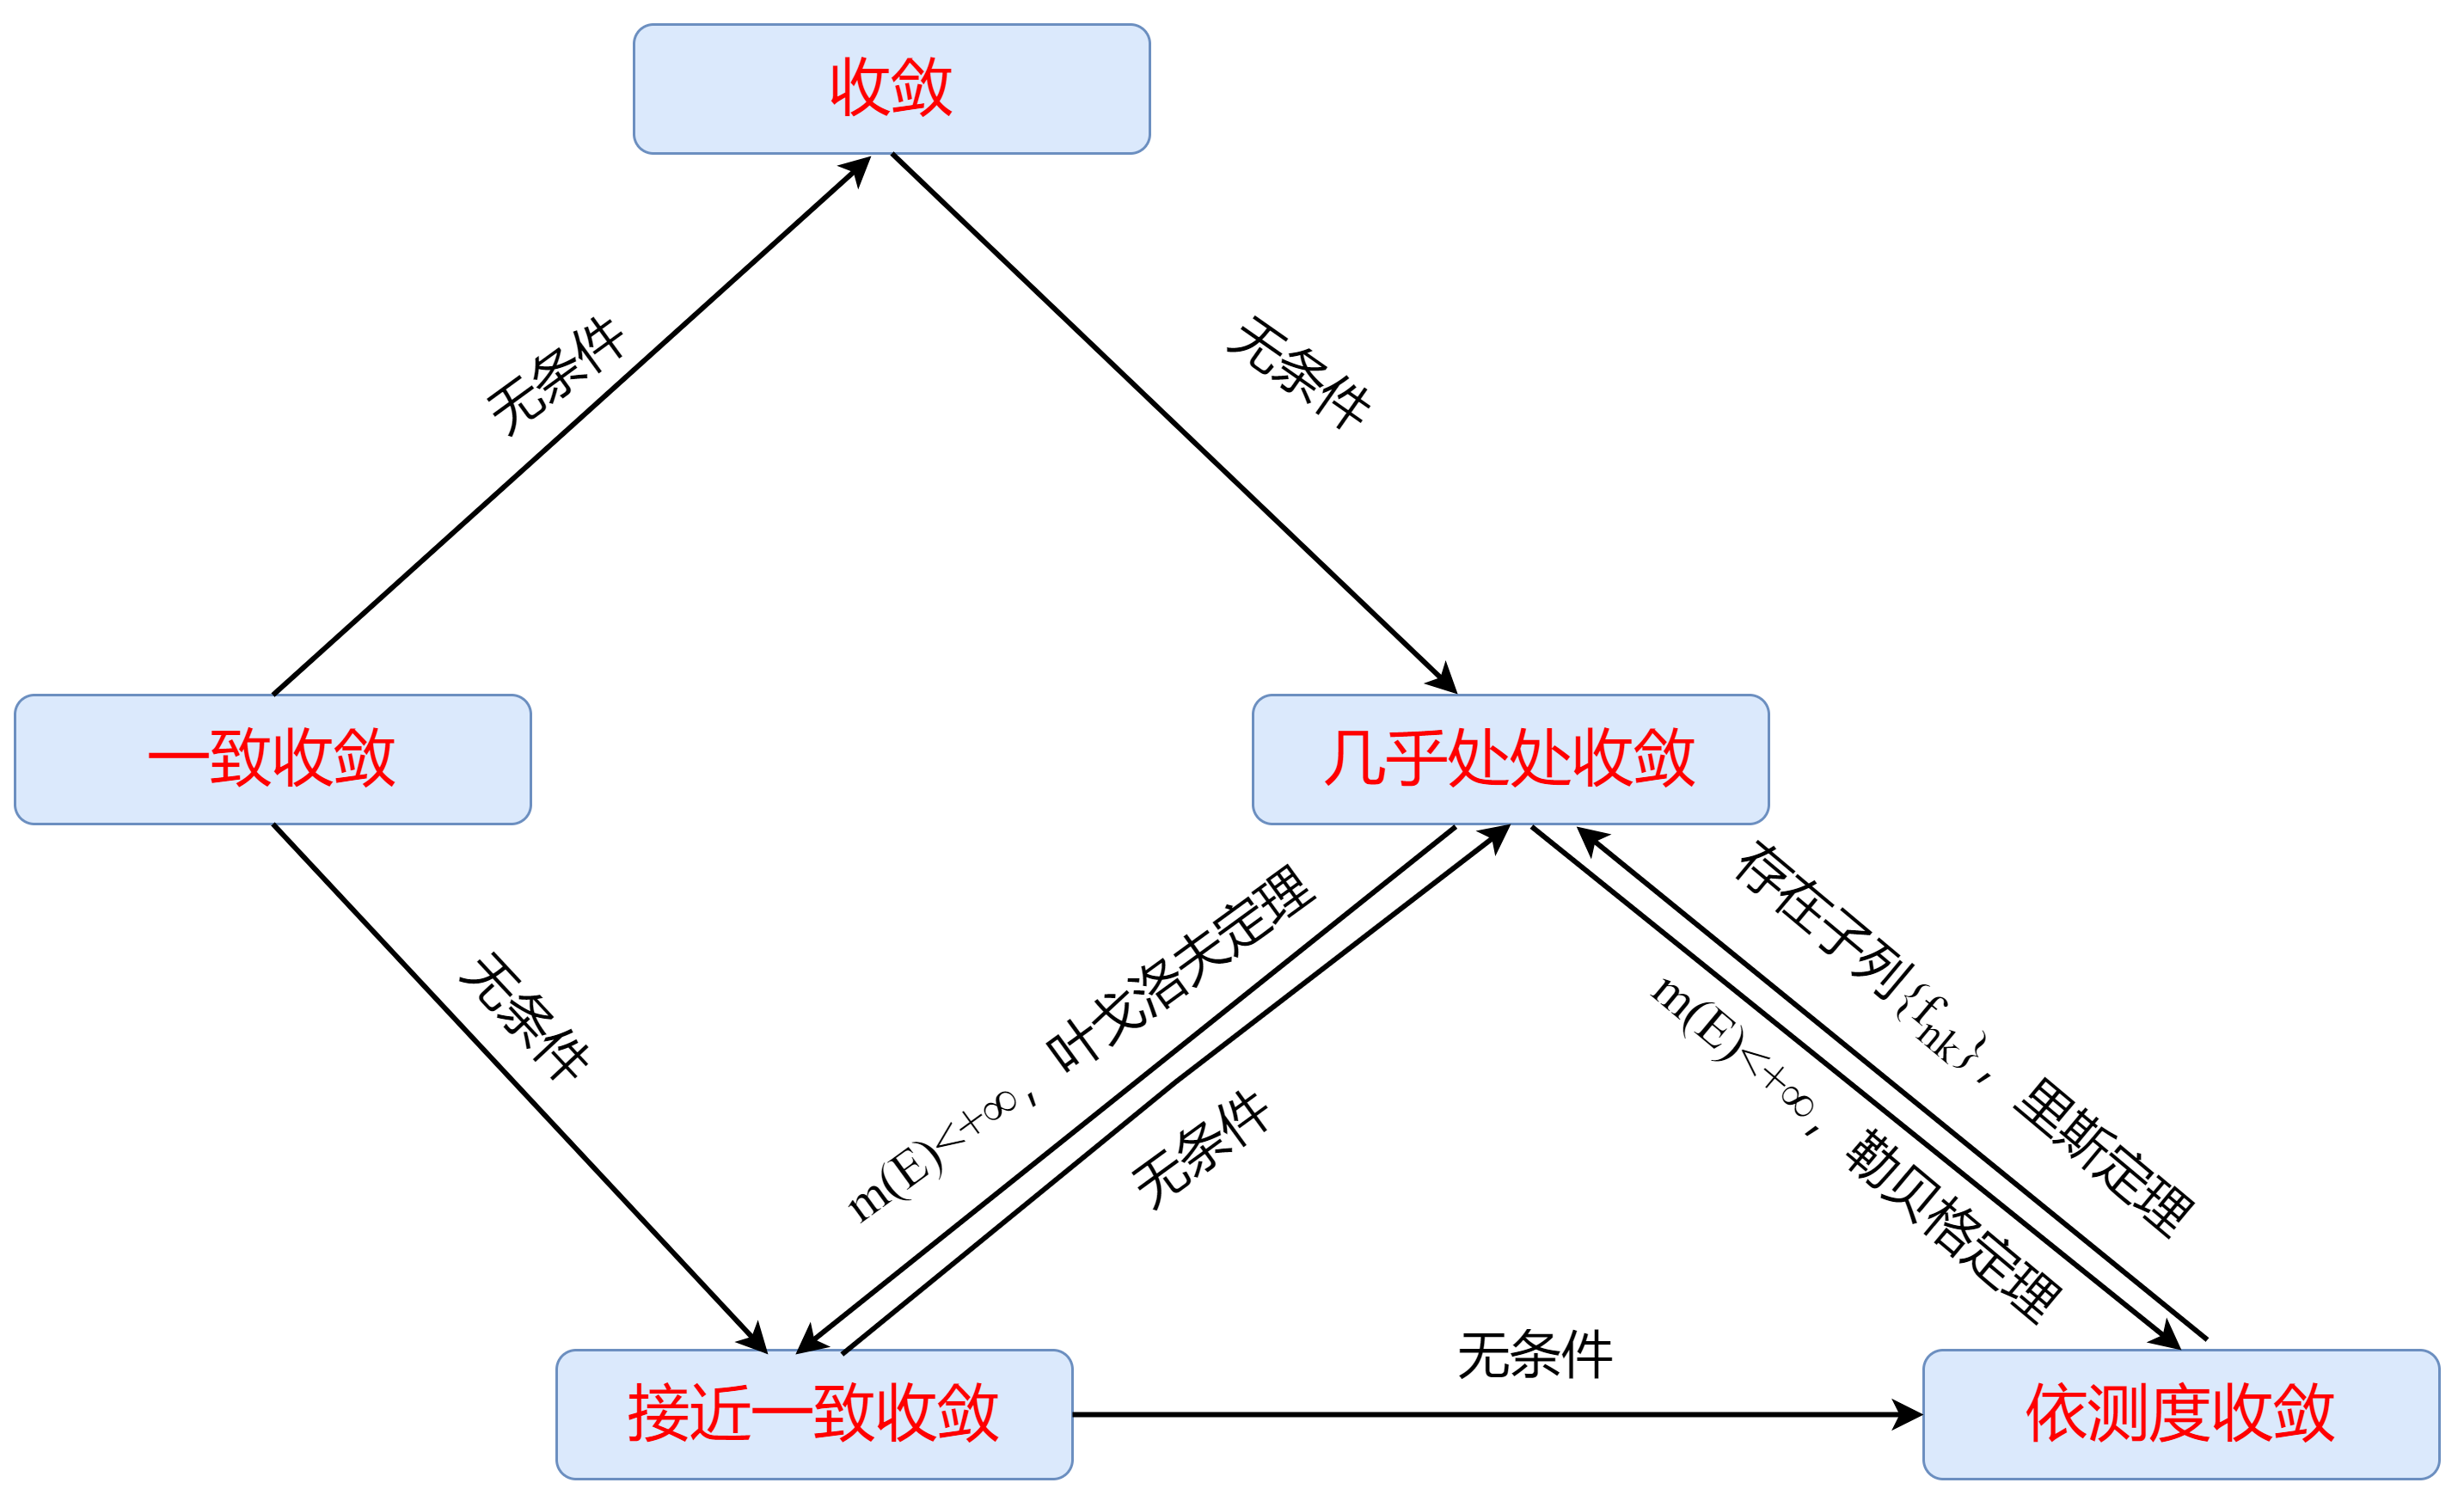
\includegraphics[scale=0.2]{几种收敛性之间的关系.png}
\caption{几种收敛性之间的关系}
\label{image:几种收敛性之间的关系}
\end{figure}


































\end{document}